\section{Introduction}

\textbf{Problem of sequential algorithm:}

\begin{itemize}
 \item design: techniques such as divide et impera, dyniamic programming, greedy, ...
 \item evaluate performance: time complexity, space complexity
 \item develop: implement with a programming language
\end{itemize}

Similarly, the same problem can be faced for Parallel and Distributed Algorithms (PDAs).

\textbf{PDAs are solved by a pool of executors, and there are two cases:}

\begin{enumerate}
 \item pool of executors such that:\\
 - have a central clock\\
 - can be share resources (i.e., memory)\\
 \begin{multicols}{2}
 [For example: Sum of 4 numbers]
  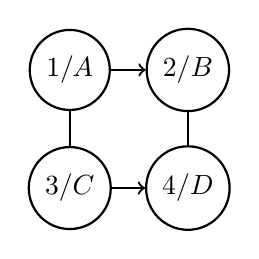
\begin{tikzpicture}[node distance={15mm}, thick, main/.style = {draw, circle}] 
   \node[main] (A)              {$1/A$}; 
   \node[main] (B) [right of=A] {$2/B$}; 
   \node[main] (C) [below of=A] {$3/C$}; 
   \node[main] (D) [below of=B] {$4/D$}; 
		
   \draw (A) -- (C);
   \draw (B) -- (D);
   \draw[->] (A) -- (B);
   \draw[->] (C) -- (D);
   \end{tikzpicture} 
		
   Number: A, B, C, D\\
   Processor: 1, 2, 3, 4\\
    \begin{algorithm}[H]
    	 \SetAlgoLined
    	 \KwIn{$G=(V,E)$}
    	 \KwResult{Sum of $V$}
     send($1$, $2$) $\rightarrow$ $A+B$\\
     send($3$, $3$) $\rightarrow$ $C+D$\\
     send($2$, $4$) $\rightarrow$ $A+B+C+D$
     \caption{Sum of 4}
	 \end{algorithm}
	 4 clock cycles
	\end{multicols}
 \item pool of executors such that:\\
 - each has its own central clock\\
 - they are connected to each outher (we cannot assume that the memory is shared)
 \begin{multicols}{2}
 [For example: Sum of 4 numbers]
  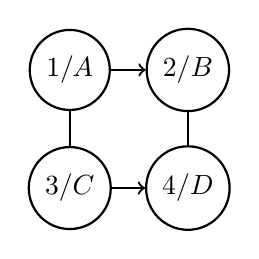
\begin{tikzpicture}[node distance={15mm}, thick, main/.style = {draw, circle}] 
   \node[main] (A)              {$1/A$}; 
   \node[main] (B) [right of=A] {$2/B$}; 
   \node[main] (C) [below of=A] {$3/C$}; 
   \node[main] (D) [below of=B] {$4/D$}; 
		
   \draw (A) -- (C);
   \draw (B) -- (D);
   \draw[->] (A) -- (B);
   \draw[->] (C) -- (D);
  \end{tikzpicture} 
		
  Number: A, B, C, D\\
  Processor: 1, 2, 3, 4\\
   \begin{algorithm}[H]
    	\SetAlgoLined
    \KwIn{$G=(V,E)$}
    \KwResult{Sum of $V$}
    send($1$, $2$) \& send($3$, $3$)\\
    // may come at different times\\
    // the processor might wait to do the final sum\\
    // could be usefull coordination signals
    \caption{Sum of 4}
   \end{algorithm}
 \end{multicols}
\end{enumerate}

In parallel algorithms the main factor is \textbf{Time}\\
- To sum 4 number the cycles are 4, but to sum 1000 number the cycles are 10\\
In distributed algorithms the main facotor is \textbf{coordination}\\
- less messages = faster

\subsection{Course Program}

For each paradigm:

\begin{enumerate}
 \item theortical model
 \item evaluate the performance
 \item simple problem to learn the techniques
\end{enumerate}

\textbf{Parallel case}

\begin{enumerate}
 \item A:
  \begin{enumerate}
   \item PRAM (immediate communication) $\rightarrow$ shared memory
   \item computing resources $\rightarrow$ time, hardware=\#processor
   \item problems:\\
    - summation\\
    - prefixed sums\\
    - sorting\\
  \end{enumerate}
 \item B:
  \begin{enumerate}
   \item shared memory model\\   
    - Linear array\\ 
    - Mesh
   \item computing resources
   \item problems:\\ 
    - Shuffle
    - Max
    - Sorting
  \end{enumerate}
\end{enumerate}

\textbf{Distributed case}

\begin{enumerate}
 \item definition of abstract  model
 \item computing resource $\rightarrow$ time, \#messages=congestion
 \item problems:\\
 - broadcast\\
 - wake up\\
 - traversal\\
 - spanning tree\\
 - election\\
 - routing
\end{enumerate}